\documentclass[final, ngerman, xcolor=pdftex, dvipsnames, table, aspectratio=169, 14pt]{beamer}
\usepackage[utf8]{inputenc}
\usepackage[ngerman]{babel}
\usepackage[T1]{fontenc}
\usepackage{droid}
\usepackage{pgf-pie}
\usepackage{hyperref}

\usepackage{pgfpages}

\setbeameroption{hide notes}

\setbeamerfont{note date}{size=\scriptsize}
\setbeamerfont{note title}{size=\footnotesize}
\setbeamerfont{note page}{size=\footnotesize}

\usepackage{graphicx}


\usetheme{DarkConsole}

\begin{document}

% The metadata of the presentation
\title[Worlds]{Worlds}
\subtitle[]{A Distributed MMO}
\author[]{Ryan Walker\footnote{\texttt{ryan.cjw@gmail.com}}}
\date{\today} % Replace with date of the presentation


\begin{frame}
  \maketitle
  \note{
    I'm the note from the title page.
  }
\end{frame}

\section*{I'm a hidden Section}
\begin{frame}{Table of Content} % This is the list of content with all the sections of the presentation
    \small 
    \tableofcontents
\end{frame}

\section{Identity}
\begin{frame}{Identity}
Worlds is the economic backbone for a distributed MMO. Is enables players to move digital assets and wealth throughout multiple games forming one massive congruent universe. 
\end{frame}

\begin{frame}{Identity}
\centering
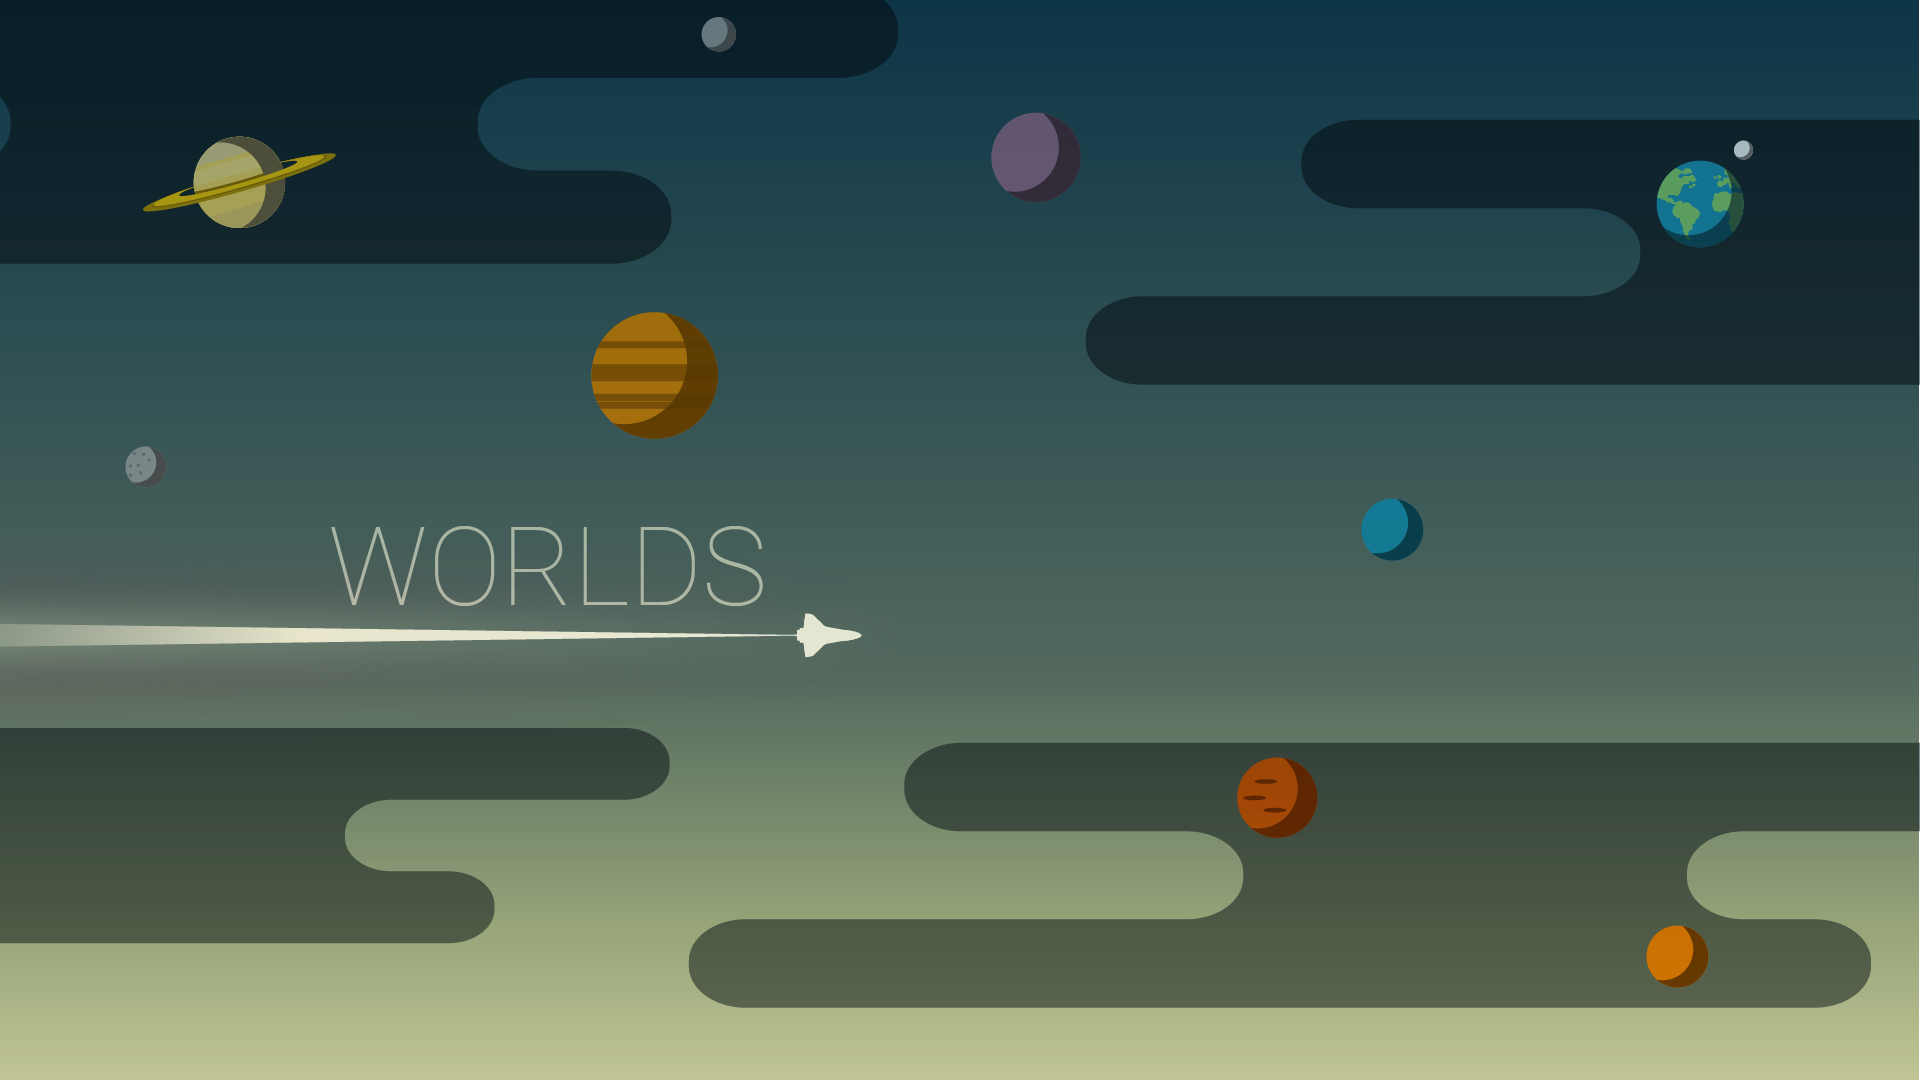
\includegraphics[scale=0.15]{Header.png} 

\textbf{Worlds} - A Distributed MMO
\end{frame}

\section{Assets}
\begin{frame}{Assets}
\href{https://www.youtube.com/watch?v=OrOZVr-j92A}{Full Stack Demo}
\\~\\

\href{https://github.com/Machine-Hum/Worlds/raw/master/Worlds-Whitepaper/whitepaper.pdf}{Whitepaper}
\\~\\

\href{worldsmmo.com}{Github}
\end{frame}

\section{Mission}
\begin{frame}{Mission}
Worlds is going to be the first open and scaleable infrastructure for building an unbounded MMO. Upon the completion on this platform, proper incentivation will lead to the organic growth of the largest online game ever created.
\end{frame}

\section{Problem}
\begin{frame}{Problem}
The economy of an open world comes down to game theory. If anyone can add code, then anyone can create unbounded resources thus creating an economic imbalance. The Worlds platform implements a smart contract to manage the resources ensuring that digital wealth cannot be created from nothing.  
\end{frame}

\section{Solution}
\begin{frame}{Solution}
Currently there are three main components to my ecosystem, the Worlds Smart Contract, the Worlds Engine (wallet) and the Minecraft fork. These three elements have been implemented and tested to demonstrate the entire stack. In the "Full Stack Demo" video listed above this is shown.
\end{frame}

\section{Target}
\begin{frame}{Target}
Initially smaller communities will be targeted, I have forked an open source version on Minecraft. The initial vision is several smaller Worlds to create a network and prove out the concept. Later on, developers will integrate their games into the universe.
\end{frame}

\section{Market}
\begin{frame}{Market}
Unlike several cyrpto projects, Worlds does not suffer from the chicken and egg problem. A small inplementation of ten or so Worlds maintained by independent parties would create an interesting experiance. The universe will scale from that.
\end{frame}

\section{Advantage}
\begin{frame}{Advantage}
My focus is full stack, by leveraging open source tech I will be able to build the game clients required to feed the initial fire. Existing project like Worlds are relying on game developers to take a leap of faith and pour valuable development time into building a game. In the beginning coding skills shouldn't be required to create a World, just someone to host a server and create the experience. 
\end{frame}

\begin{frame}{Advantage}
My platform is 100\% open source and transparent. I want to build tools to enable my vision, and then use those tools to show people what's possible.
\end{frame}

\begin{frame}{Advantage}
Worlds is built on EOS, therefor it has the rapid finality required for a game. 
\end{frame}

\begin{frame}{Disadvantages}
Marketing is a necessary evil. I believe that strong marketing without strong tech is a fundraising mechanism. While strong marketing with strong tech is a community building mechanism. I have been focusing on the technology up until now, however in the future once I build out the tools there will be a requirement for marketing. Without funding, success will be difficult.  
\end{frame}

\section{Roadmap}
\begin{frame}{Roadmap}
\begin{itemize}
\small
\item{5/2018} Project conceptualised, first commit.
\item{9/2018} Paper Complete, EOS blockchain selected.
\item{1/2019} First item created on local testnet.
\item{5/2019} Wallet/Engine Functional.
\item{6/2019} Full stack functional test.
\item{1/2020} Test net deployment.
\item{3/2020} First World (Realm.one) deployment.
\item{6/2020} Main net deployment.
\end{itemize}

\end{frame}

\section{Buisness / Token Model}
\begin{frame}{Token Cap Table}

\begin{center}

\begin{tikzpicture}
\footnotesize
\pie [rotate = 180, radius=1.5, color={indigo}, explode=0.2]
{10/Kept for team,
 40/Given to developers, 
 10/Sold to Private Investment,
 40/Community Airdrop
}
\end{tikzpicture}
\\
\end{center}
The token cap model is geared towards stimulating initial project growth within the community.
\end{frame}

\section{Fundraising}

\begin{frame}{Fundraising}
\begin{center}
\begin{tikzpicture}
\footnotesize
\pie [square, radius=2.9, text=legend, after number = {k}, color={indigo, red, green, blue, purple, pink, orange, black}, sum=160]
{55/Personal Wage,
 10/Office Space, 
 5/Graphic Design,
 45/Contract Game Developers,
 20/UI and UX ,
 10/Concept Art,
 5/Web Development,
 10/Server Fees
}
\end{tikzpicture}

Fundraising target for the first year of development: \$160k.
\end{center}

\end{frame}
\begin{frame}{Fundraising}
Until now, the development has been on my free time. I'm looking to raise seed funding to make this my full time job. Above is the breakdown for one year of development. I am currently offering 5\% of the token cap table of WOR. Following the depletion of funding I will be aiming to raise a series A.
\end{frame}

\begin{frame}{Thanks}
I greatly appriciate your consideration, I hope you have gained a better understanding of my project and can share the same vision. If you havn't watched the demo video, I would encurage yo to do so. Do not hesitate to reach out with further questions.
\\~\\
\begin{center}
Ryan Walker - Ryan.cjw@gmail.com
\end{center}
\end{frame}

\end{document}
